%%%%%%%%%%Second Chapter%%%%%%%%%%
\chapter{Theoretical Background}

\section{Antenna Theory}

\section{Metasurface Transmitarray Lens Antenna}
This section presents a paraphrased synthesis of the transmitarray antenna concepts discussed by Abdelrahman et al.~\cite{Abdelrahman2017} and relates them to metasurface transmitarray lens antennas. A transmitarray antenna consists of an illuminating feed source and a thin transmitting surface composed of antenna elements or metasurface unit cells. The feed is placed at an equivalent focal point, causing the incident wave on the aperture to have a spherical phase front.

Each element on the transmitting surface is designed with a specific transmission coefficient to control the transmitted phase. By compensating for the different path lengths from the feed to each element, the transmitarray converts the spherical phase front into a more planar transmitted phase front and forms a directive beam with higher gain. This makes transmitarray antennas useful for compact wireless communication, remote sensing, terahertz imaging, and other applications requiring controlled high-gain radiation.

\subsection{Unit-Cell Element Analysis}
The performance of a transmitarray is strongly influenced by the design of its individual unit-cell elements, since each element must provide a controlled transmission phase while maintaining adequate transmission magnitude. In a metasurface transmitarray lens antenna, the unit cell is therefore analyzed not only as a physical geometry, but also as a phase-control element that determines how the incident wave from the feed is transformed after passing through the aperture.

The transmission characteristics of a unit cell are commonly evaluated through a parametric study, where selected geometrical dimensions are varied and the resulting phase and magnitude responses are observed. In electromagnetic simulation, the unit cell can be modeled with periodic boundary conditions to approximate its behavior inside a larger array. This approach allows the designer to estimate the phase range, transmission loss, and sensitivity of the element before constructing the complete transmitarray aperture. A suitable unit-cell design should provide a broad phase variation, preferably close to a full $360^\circ$ range, while keeping the transmission magnitude as high and stable as possible~\cite{Abdelrahman2017}.

In this thesis, the unit-cell candidate is selected using the power conservation principle, where the incident power is divided into reflection, transmission, and loss:
\begin{equation}
    \left|S_{11}\right|^2 + \left|S_{21}\right|^2 + P_{\mathrm{loss}} = 1,
\end{equation}
\begin{equation}
    P_R = \left|S_{11}\right|^2 = 10^{S_{11,\mathrm{dB}}/10}, \qquad
    P_T = \left|S_{21}\right|^2 = 10^{S_{21,\mathrm{dB}}/10}.
\end{equation}
Here, $S_{11}$ and $S_{21}$ represent the reflection and transmission coefficients, respectively. Therefore, the preferred element is the one with high transmitted power, low reflected power, low loss, and the required transmission phase response.



\subsection{Antenna Lens Design}
The antenna lens design in this thesis is formulated based on phase compensation principles and transmitarray lens design approaches reported in~\cite{RezkiElArif2023,Al-Joumayly2011,Abdelrahman2017}. The main purpose of the lens is to compensate for the phase difference of the spherical wavefront radiated by the feed source. Because the feed is placed at a finite focal distance, the incident wave reaches different positions on the aperture through different path lengths. Therefore, the aperture must provide a spatially varying transmission phase so that the transmitted fields become approximately phase-aligned after passing through the lens. This design concept is illustrated in Fig.~\ref{fig:antenna-lens-views}.

\begin{figure}[htbp]
    \centering
    \begin{subfigure}[t]{0.48\textwidth}
        \centering
        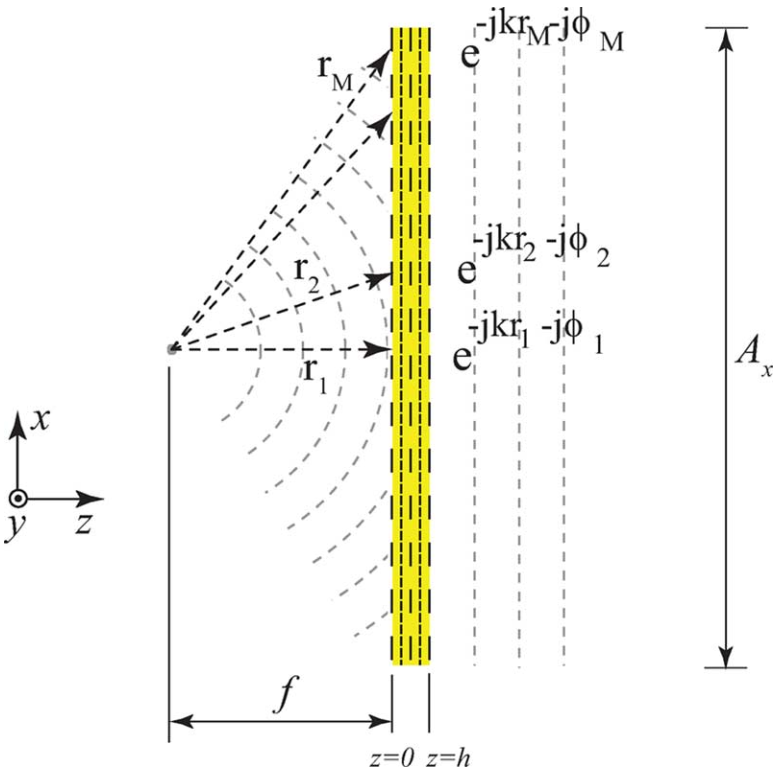
\includegraphics[width=\textwidth]{Images/AntennaLensSideView.PNG}
        \caption{Side view}
        \label{fig:antenna-lens-side-view}
    \end{subfigure}
    \hfill
    \begin{subfigure}[t]{0.48\textwidth}
        \centering
        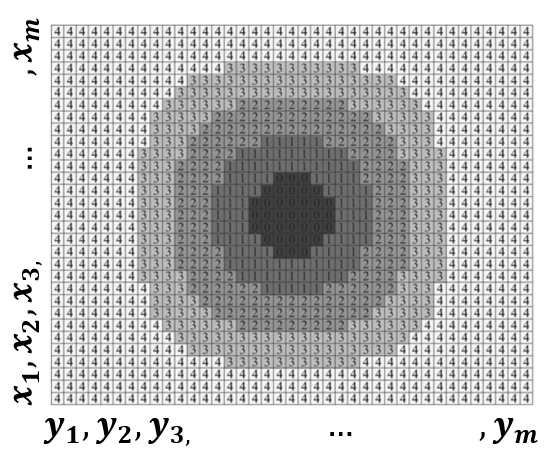
\includegraphics[width=\textwidth]{Images/AntennaLensFrontView.PNG}
        \caption{Front view}
        \label{fig:antenna-lens-front-view}
    \end{subfigure}
    \caption{Antenna lens illustrations showing the feed-to-aperture path-length differences in the side view and the aperture zoning in the front view.}
    \label{fig:antenna-lens-views}
\end{figure}

Figure~\ref{fig:antenna-lens-views}(a) shows the side view of the lens configuration, where the feed illuminates the aperture from the focal position and produces different propagation paths toward different parts of the lens. Figure~\ref{fig:antenna-lens-views}(b) shows the front view of the aperture, where the lens is implemented as a two-dimensional unit-cell array. The numbered regions indicate that the aperture is grouped into concentric phase zones, so unit cells within the same zone can use the same phase-shifter type. This discretized zoning approximates the continuous phase profile required for lens operation while keeping the physical implementation simpler.

For the phase calculation, the aperture is divided into $M$ concentric zones indexed by $m$, where $m=0,1,\ldots,M-1$. If the center of zone $m$ is located at $(x_m,y_m,z=0)$, the required transmission phase for the unit cells in that zone is calculated as
\begin{equation}
    \Phi(x_m,y_m) =
    -k_0(r_m - f)
    + k_0\left(\sqrt{(A/2)^2 + f^2} - f\right)
    + \Phi_0.
\end{equation}
In this expression, $\Phi(x_m,y_m)$ denotes the desired transmission phase at the center of zone $m$, $k_0=2\pi/\lambda_0$ is the free-space wavenumber, $\lambda_0$ is the free-space wavelength, $r_m$ is the distance from the feed point to the center of zone $m$, $f$ is the focal distance, $A$ is the aperture size, and $\Phi_0$ is a positive constant phase delay applied to all unit-cell responses. The resulting phase values are then used as the design targets for selecting and arranging the unit-cell elements across the lens aperture.

\section{Wireless Channel}
This thesis evaluates the wireless channel to examine how the antenna lens modifies the end-to-end electromagnetic response between multiple transmit and receive positions. Following the general wireless communication framework described by Tse and Viswanath~\cite{Tse2005}, the analysis is not limited to received power, but also considers how the lens affects angular separation, spatial multiplexing behavior, and the correlation between propagation paths. For this purpose, the measured or simulated S-parameters are treated as a frequency-domain representation of the communication channel, allowing the with-lens and without-lens cases to be compared in a consistent manner.

\subsection{Formulation Wireless Channel}
In a general multiple-input multiple-output (MIMO) system, the wireless channel connects $N_T$ transmit ports to $N_R$ receive ports. At each frequency point $f$, the channel response can be represented by a complex matrix
\begin{equation}
    \mathbf{H}(f) \in \mathrm{C}^{N_R \times N_T},
\end{equation}
where each row corresponds to a receive port and each column corresponds to a transmit port. When the channel is obtained from electromagnetic simulation or network-analyzer measurement, each element of the matrix can be constructed from the transmission S-parameter between the corresponding transmit and receive ports:
\begin{equation}
    H_{ij}(f) = S(\mathrm{rx}_i,\mathrm{tx}_j;f),
\end{equation}
where $H_{ij}(f)$ denotes the channel coefficient from the $j$-th transmit port to the $i$-th receive port at frequency $f$.

The corresponding frequency-domain input-output relationship is written as
\begin{equation}
    \mathbf{y}(f) = \mathbf{H}(f)\mathbf{x}(f) + \mathbf{n}(f),
\end{equation}
where $\mathbf{x}(f)\in\mathrm{C}^{N_T \times 1}$ is the transmitted signal vector, $\mathbf{y}(f)\in\mathrm{C}^{N_R \times 1}$ is the received signal vector, and $\mathbf{n}(f)$ is the additive noise vector. For example, in a $3\times3$ configuration, the channel matrix becomes
\begin{equation}
    \mathbf{H}(f) =
    \begin{bmatrix}
        S(\mathrm{rx}_1,\mathrm{tx}_1;f) & S(\mathrm{rx}_1,\mathrm{tx}_2;f) & S(\mathrm{rx}_1,\mathrm{tx}_3;f) \\
        S(\mathrm{rx}_2,\mathrm{tx}_1;f) & S(\mathrm{rx}_2,\mathrm{tx}_2;f) & S(\mathrm{rx}_2,\mathrm{tx}_3;f) \\
        S(\mathrm{rx}_3,\mathrm{tx}_1;f) & S(\mathrm{rx}_3,\mathrm{tx}_2;f) & S(\mathrm{rx}_3,\mathrm{tx}_3;f)
    \end{bmatrix}.
\end{equation}
In this formulation, $\mathbf{H}(f)$ represents the measured or simulated end-to-end RF channel response. It therefore includes not only free-space propagation, but also the effects of the transmit antenna, receive antenna, antenna lens response, propagation path, mutual coupling, impedance mismatch, and measurement reference planes. This makes the S-parameter-based matrix suitable for empirical channel evaluation in the antenna-lens-assisted MIMO system.

\subsection{Singular Value Decomposition of the Channel Matrix}
After the channel matrix is constructed, singular value decomposition (SVD) is applied to $\mathbf{H}(f)$ at each frequency point. This decomposition expresses the MIMO channel as
\begin{equation}
    \mathbf{H}(f) = \mathbf{U}(f)\mathbf{\Sigma}(f)\mathbf{V}^{H}(f),
\end{equation}
where $\mathbf{U}(f)$ and $\mathbf{V}(f)$ are unitary matrices, $\mathbf{V}^{H}(f)$ denotes the Hermitian transpose of $\mathbf{V}(f)$, and $\mathbf{\Sigma}(f)$ contains the singular values of the channel matrix. For the $3\times3$ channel example used in this thesis, the singular-value matrix can be written as
\begin{equation}
    \mathbf{\Sigma}(f) =
    \mathrm{diag}\left(\sigma_1(f),\sigma_2(f),\sigma_3(f)\right),
\end{equation}
with
\begin{equation}
    \sigma_1(f) \geq \sigma_2(f) \geq \sigma_3(f) \geq 0.
\end{equation}
The singular value $\sigma_i(f)$ represents the amplitude gain of the $i$-th equivalent parallel MIMO eigenchannel, while $\sigma_i^2(f)$ represents its corresponding power gain. If only $\sigma_1(f)$ is dominant, the channel is mainly supported by one spatial mode. In contrast, when $\sigma_1(f)$, $\sigma_2(f)$, and $\sigma_3(f)$ have comparable values, the channel provides better spatial multiplexing capability.

Two additional indicators are extracted from the same singular values. The condition number is used to evaluate the balance among the MIMO eigenchannels:
\begin{equation}
    \kappa(f) = \frac{\sigma_1(f)}{\sigma_3(f)}.
\end{equation}
A lower $\kappa(f)$ indicates that the channel modes are more balanced. The effective rank is then used to estimate the effective number of active spatial modes:
\begin{equation}
    p_i(f) =
    \frac{\sigma_i^2(f)}{\sum_{k=1}^{3}\sigma_k^2(f)},
    \qquad
    r_{\mathrm{eff}}(f) =
    \exp\left(-\sum_{i=1}^{3}p_i(f)\ln p_i(f)\right).
\end{equation}
For a $3\times3$ channel, $r_{\mathrm{eff}}(f)$ ranges from 1 to 3. A value closer to 3 indicates that more spatial modes contribute to the channel response, while a value closer to 1 indicates that the channel is dominated by fewer modes.
